\subsection{Label blobs}
\label{sec:labelblobs}

Om het benodigde object te detecteren is het nodig om ieder object te
identificeren. De makkelijkste manier om dit te doen is door ieder object een
nummer te geven. Zo kunnen van alle nummers de eigenschappen bepaald worden.

Deze operator is het meest complex en heeft dus ook de meeste tijd nodig.
Gelukkig is er voldoende ruimte voor snelheidsverbetering.

Door er voor te zorgen dat alle blobs een maximale waarde hebben kan er voorkomen
worden dat er nummer conflicten optreden. Daarvoor is het dus belangrijk eerst
alle pixels op 255 te zetten.

Vervolgens moet iedere pixel van 255 een nummer krijgen. Door het plaatje van
links boven naar rechts onder te doorlopen worden de blobs gelabeld. Door bij
iedere pixel te controleren of ze al een gelabelde pixel buur-pixel hebben
probeert het programma te voorkomen dat 1 blob 2 labels krijgt. Helaas is dit
niet helemaal te voorkomen (figuur \ref{fig:lbstep1}).

\begin{figure}
    \begin{center}
        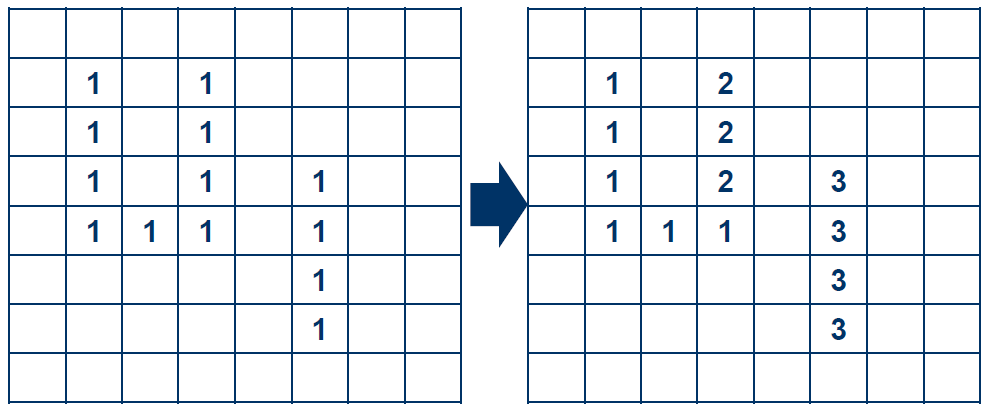
\includegraphics[scale=0.4]{figures/label_blobs_step1.png}
    \end{center}
    \caption{Verkeerd gelabelde blobs na de 1ste iteratie.}
    \label{fig:lbstep1}
\end{figure}

Het eerste label proces is redelijk complex omdat er gecontroleerd moet worden
of een blob al gelabeld is met een lager nummer ondanks dat al meerdere blobs gelabeld
zijn (listing \ref{lst:labeling1}).

\begin{listing}
    \begin{minted}{c}
      if(imgArr[h][w] == 255){
        blobDetected = 1;
        if (iNeighbourCount(img, w, h, blobCount, connected)) {
            imgArr[h][w] = blobCount;
        } else {
            for (j = blobCount; j != 0; j--) {
                if(iNeighbourCount(img, w, h, j, connected)){
                    foundFlag = 1;
                    break;
                }
            }

            if (foundFlag) {
                imgArr[h][w] = j;
                foundFlag = 0;
            } else {
                blobCount += 1;
                imgArr[h][w] = blobCount;
            }

        }
    }
    \end{minted}
    \caption{Het labelen van blobs}
    \label{lst:labeling1}
\end{listing}

\texttt{blobDetected} wordt gebruikt als controle of er überhaupt wel een blob
in het plaatje is. Zo niet, dan kan er na deze iteratie ook gestopt worden met
de functie.

Vervolgens dient de dubbel gelabelde 1 label te krijgen. Dit is te bereiken
door te beginnen in de rechter onder hoek en zo naar links boven te werken.
Door iedere keer te kijken naar de pixels achter en onder het huidige pixel
kan de laagste waarde van de pixel worden bepaald. Het is uiteraard wel
belangrijk om rekening te houden met het x connected verhaal.
Daarna wordt hetzelfde gedaan alleen dan van de linker boven hoek naar de
rechter onder hoek. En tot slot wordt er gecontroleerd of alle blobs nu
maar 1 label hebben, zo niet, dan herhaalt het proces zich nog eens (zie
figuur \ref{fig:lbstep2}).

\begin{figure}
    \begin{center}
        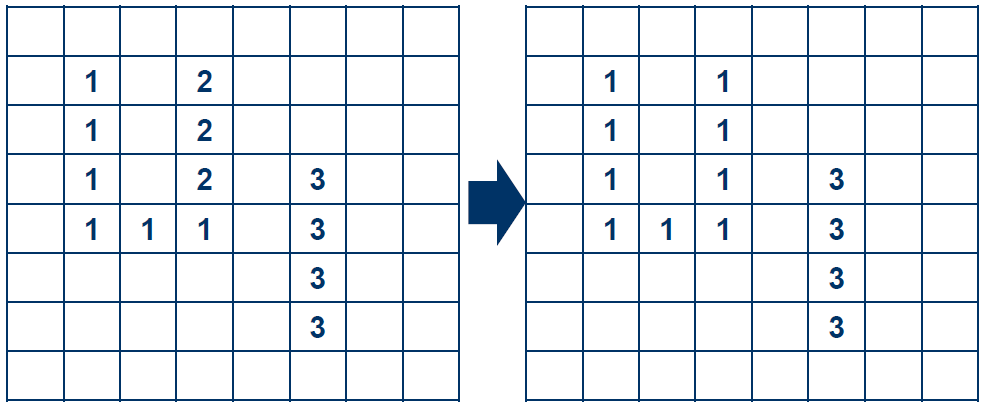
\includegraphics[scale=0.4]{figures/label_blobs_step2.png}
    \end{center}
    \caption{Uniform gelabelde blobs na (verschillende) iteraties.}
    \label{fig:lbstep2}
\end{figure}

Nu zijn er alleen gaten in de nummering. Dit kan opgelost worden door nog
één extra keer over het plaatje te gaan en de blobs te labelen van links
boven naar rechts onder. Door een teller bij te houden kunnen de correct
gelabelde blobs automatisch worden genegeerd.
